\documentclass[10pt,conference]{IEEEtran}
\usepackage[T1]{fontenc}
\usepackage{textcomp}
\usepackage{amsmath}
\usepackage{booktabs}
\usepackage{cite}
\usepackage{url}
\usepackage{tikz}
\usetikzlibrary{arrows.meta,positioning}

\title{BasketIQ: Retail Basket Recommendations and RFM Customer Segmentation with Association Mining}
\author{\IEEEauthorblockN{Sukumar Sawant, Rohit Soneji, Piyush Gupta}
\IEEEauthorblockA{Department of Computer Engineering\\
Vidyalankar Institute of Technology, Mumbai, India\\
Student IDs: 24102B0049, 24102B0059, 24102B0054}}

\begin{document}
\maketitle

\begin{abstract}
BasketIQ is a retail analytics application that combines product-pair discovery, customer segmentation, and a browsable marketplace. It is built around the UCI Online Retail transaction data. The project workflow removes duplicate rows, cancelled invoices, non-positive quantities and prices, and transactions without a customer identifier, leaving 392,692 line items. Two association mining methods are exposed for product recommendations: Apriori, whose saved artifact contains 190 rules generated at a minimum support of 0.015 and filtered at lift 1.2, and FP-Growth, which mines the transaction matrix on demand. Customer behavior is summarized with recency, frequency, and monetary value (RFM); a log-transformed, standardized K-Means model assigns 4,338 customers to four segments. The dashboard connects these analyses with sales charts, rule exploration, and a marketplace demonstration that offers a simulated 10\% discount on recommended add-on products. The application is a decision-support prototype rather than a live commerce system. In particular, the stored artifacts do not contain a controlled runtime comparison between Apriori and FP-Growth, nor an external validation of the clusters. The paper describes the implemented workflow and reports only results verifiable from the supplied data and model artifacts.
\end{abstract}

\begin{IEEEkeywords}
Retail analytics, market basket analysis, Apriori, FP-Growth, customer segmentation, RFM, K-Means
\end{IEEEkeywords}

\section{Introduction}
Retail transaction records can support two useful but different analyses. Market basket analysis identifies products that occur together in invoices and can suggest complementary items. Customer segmentation instead groups people with similar purchasing histories so that analysts can distinguish recent, frequent, and high-value customers. Presenting these analyses in separate notebooks makes it harder to relate them to practical retail decisions.

BasketIQ integrates the two tasks in a single web application. Its association-rule workflow uses Apriori as the saved rule catalogue and FP-Growth as an alternative frequent-pattern miner. The K-Means workflow groups customers from RFM features. A dashboard presents sales summaries and segment profiles, while the marketplace uses basket recommendations to demonstrate add-on offers. The project does not train a supervised purchase-propensity model: association rules summarize co-occurrence and should not be interpreted as causal effects or individualized purchase probabilities.

The contributions are an integrated analytics workflow, an implementation of two frequent-pattern approaches on the same invoice-item data, and an RFM-based customer segmentation view. We document the current artifacts and distinguish stored evaluation evidence from capabilities that have not been benchmarked.

\section{Dataset and Preparation}
The dataset is the UCI Online Retail collection, containing transactions from a UK-based, non-store retailer between December 1, 2010 and December 9, 2011 \cite{uci}. The supplied source contains 541,909 transaction rows. The project preprocessing removes 5,268 duplicate rows, 9,251 cancelled invoices, 1,336 rows with non-positive quantities, 1,176 rows with non-positive unit prices, and 132,186 rows with missing customer identifiers. The resulting cleaned file contains 392,692 line items. Customer identifiers are converted to integers, descriptions are trimmed and uppercased, invoice dates are parsed, and line revenue is derived as quantity multiplied by unit price.

For association mining, each invoice is represented as a set of distinct product descriptions. Quantity does not create repeated items in the binary transaction matrix: an item is present when it occurs in the invoice. This representation matches the basket-level interpretation of support. For customer segmentation, transactions are aggregated by customer. Recency is the number of days from the latest transaction date to the dataset reference date; frequency is the number of distinct invoices; monetary value is total line revenue. The stored customer table has 4,338 customers and the product catalogue has 3,665 distinct stock codes.

\section{System Architecture}
The frontend is a React application. An Express service exposes analytics and product endpoints and calls Python for data processing and model inference. Pandas and NumPy prepare summaries; mlxtend supplies the frequent-pattern algorithms; scikit-learn supplies K-Means and feature scaling. CSV artifacts store the cleaned transactions, product catalogue, customer segment assignments, and Apriori rules. Apriori results and K-Means segments are loaded from saved files. FP-Growth constructs a binary invoice-item matrix and mines frequent itemsets when the user selects that method.

\begin{figure*}[t]
\centering
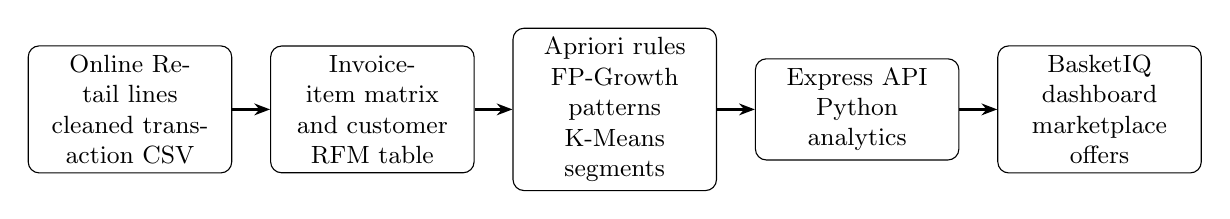
\begin{tikzpicture}[node distance=0.42cm and 0.48cm,
 b/.style={draw,rounded corners,align=center,minimum height=0.82cm,text width=2.35cm,font=\small},
 a/.style={-{Stealth[length=2mm]},thick}]
\node[b] (data) {Online Retail lines\\cleaned transaction CSV};
\node[b,right=of data] (basket) {Invoice-item matrix\\and customer RFM table};
\node[b,right=of basket] (mining) {Apriori rules\\FP-Growth patterns\\K-Means segments};
\node[b,right=of mining] (api) {Express API\\Python analytics};
\node[b,right=of api] (app) {BasketIQ dashboard\\marketplace offers};
\draw[a] (data)--(basket); \draw[a] (basket)--(mining); \draw[a] (mining)--(api); \draw[a] (api)--(app);
\end{tikzpicture}
\caption{Implemented data flow from cleaned retail transactions to mining outputs and the interactive application.}
\label{fig:architecture}
\end{figure*}

\section{Mining Methods}
\subsection{Apriori Association Rules}
Apriori uses the downward-closure property: every subset of a frequent itemset must also be frequent. It counts candidate itemsets in progressively larger levels and prunes candidates whose subsets are infrequent \cite{agrawal}. For itemsets $X$ and $Y$, the application uses support, confidence, and lift:
\begin{equation}
\operatorname{supp}(X\Rightarrow Y)=P(X\cup Y),\quad
\operatorname{conf}(X\Rightarrow Y)=\frac{P(X\cup Y)}{P(X)},\quad
\operatorname{lift}(X\Rightarrow Y)=\frac{P(X\cup Y)}{P(X)P(Y)}.
\end{equation}
The training notebook sets minimum support to 0.015 and keeps rules with lift at least 1.2. These thresholds determine which patterns are retained; they are not predictive accuracy measures.

\subsection{FP-Growth Recommendation}
FP-Growth orders frequent items, compresses transactions into an FP-tree, and mines conditional pattern bases without generating the same candidate levels as Apriori \cite{han}. In the application it accepts the selected basket, support, and confidence thresholds, builds a Boolean invoice-item matrix from cleaned rows, mines frequent patterns, derives association rules, and returns consequents not already in the basket. The frontend can display either algorithm's complementary-item suggestions. The stored project results do not include a fixed FP-Growth rule export or a matched timing and memory study, so we make no claim that one implementation is faster here.

\subsection{RFM K-Means Segmentation}
The customer feature vector is $\mathbf{x}_i=(R_i,F_i,M_i)$, where the three values denote recency, frequency, and monetary value. The workflow applies $\log(1+x)$ to reduce skew and standardizes the features before fitting K-Means with $K=4$, ten initializations, and random seed 42. K-Means iteratively assigns each point to its nearest centroid and updates each centroid to the mean of its assigned points, minimizing the within-cluster sum of squared distances \cite{macqueen}:
\begin{equation}
J=\sum_{i=1}^{n}\min_{1\leq k\leq4}\|\mathbf{z}_i-\boldsymbol{\mu}_k\|_2^2.
\end{equation}
Cluster numbers have no inherent ordering; the business labels are assigned after examining the segment means.

\section{Results and Application}
The saved Apriori CSV contains 190 rules; the project README records 442 frequent itemsets at the stated support threshold. The customer segment artifact contains all 4,338 customers. Table~\ref{tab:segments} summarizes the stored cluster profiles. The segments are uneven: the inactive group is the largest, while the high-value group has the greatest mean monetary value and order frequency. These are descriptive differences in this historical dataset, not evidence that a particular marketing action will cause higher revenue.

\begin{table}[t]
\centering
\caption{Stored K-Means RFM segment profiles}
\label{tab:segments}
\small
\begin{tabular}{lrrrr}
\toprule
Segment & $n$ & Recency & Frequency & Monetary (\pounds)\\
\midrule
VIP / high value & 713 & 12.17 & 13.75 & 8,088.02\\
Lost / inactive & 1,622 & 181.51 & 1.32 & 341.00\\
New / recent & 837 & 17.70 & 2.19 & 557.32\\
Loyal regular & 1,166 & 71.64 & 4.08 & 1,801.78\\
\bottomrule
\end{tabular}
\end{table}

The user interface includes an overview of revenue, transactions, customers, products, and monthly trends; a basket analysis view with an algorithm selector; an association-rule explorer; and customer segment profiles. The marketplace retrieves products and historical unit-price values from the project catalogue. When the user adds a product, Apriori rules can suggest a related item. Adding a suggested item applies a 10\% discount to that line in the displayed basket estimate. This promotion is a front-end demonstration only: the dataset contains no current prices, stock availability, coupon policy, checkout, or payment service.

\section{Limitations and Conclusion}
The project demonstrates complementary descriptive methods rather than a controlled algorithm contest. The Apriori artifact uses a fixed support threshold and has 190 exported rules, whereas FP-Growth mines on demand with request thresholds. A fair speed or quality comparison would require identical transaction encodings, thresholds, rule filters, hardware, repeated runs, and recorded output metrics. Such results are not currently stored. Similarly, the model artifacts do not retain silhouette scores or a resampling-based cluster stability assessment; K-Means quality should not be inferred solely from four interpretable segment means.

The source data represent one UK retailer over roughly one year and contain no live browsing, stock, or response-to-promotion data. The 10\% offer is therefore a simulated interface behavior, not a tested uplift strategy. Future work should persist FP-Growth outputs and runtime metadata, compare the algorithms on the same baskets, assess cluster stability and alternative values of $K$, and evaluate offers using a randomized experiment with current prices and observed outcomes.

BasketIQ brings Apriori, FP-Growth, and RFM K-Means into a single retail analytics product. The saved artifacts support 190 association rules and four customer segments, while on-demand FP-Growth provides a second pattern-mining path. The dashboard and marketplace make these outputs easier to inspect, but any operational recommendation or discount campaign requires validation beyond the historical dataset.

\begin{thebibliography}{8}
\bibitem{uci}
D. Chen, ``Online Retail,'' UCI Machine Learning Repository, 2015, doi: 10.24432/C5BW33.

\bibitem{agrawal}
R. Agrawal and R. Srikant, ``Fast algorithms for mining association rules in large databases,'' in \emph{Proc. 20th Int. Conf. Very Large Data Bases}, 1994, pp. 487--499.

\bibitem{han}
J. Han, J. Pei, and Y. Yin, ``Mining frequent patterns without candidate generation,'' \emph{SIGMOD Record}, vol. 29, no. 2, pp. 1--12, 2000, doi: 10.1145/335191.335372.

\bibitem{macqueen}
J. MacQueen, ``Some methods for classification and analysis of multivariate observations,'' in \emph{Proc. Fifth Berkeley Symp. Mathematical Statistics and Probability}, vol. 1, 1967, pp. 281--297.

\bibitem{pedregosa}
F. Pedregosa \emph{et al.}, ``Scikit-learn: Machine learning in Python,'' \emph{J. Mach. Learn. Res.}, vol. 12, pp. 2825--2830, 2011.

\bibitem{raschka}
S. Raschka, ``MLxtend: Providing machine learning and data science utilities and extensions to Python's scientific computing stack,'' \emph{J. Open Source Software}, vol. 3, no. 24, p. 638, 2018, doi: 10.21105/joss.00638.
\end{thebibliography}

\end{document}
